\section{Data Analysis for Compact Binary Coalescence Signals}\label{sec:cbc_searches}
The observable changes that \acrshort{gw}s induce in detectors are very small, as we will see in section \ref{sec:detectors}. Consequently, detecting them directly is a difficult problem that stood unsolved for nearly a century.

The first indirect detection of \acrshort{gw}s was made in 1982 when Joseph H. Taylor and Joel M. Weisberg closely studied the pulsar PSR 1913+16~\cite{Taylor:1982zz}. Said pulsar was discovered in 1974 and was the first one that was part of a binary system~\cite{Hulse:1974eb}. It became known as the Hulse-Taylor pulsar, named after the researchers who discovered it. A pulsar is a rotating \acrshort{ns} that emits a beam of radiation. If the beam continuously sweeps across a detector, it appears as a periodic signal. The frequency of these pulses is known to be extremely stable~\cite{Matsakis:1997aaa, Verbiest:2009aaa} and, consequently, allows to trace the orbit of pulsars in binaries very accurately. As was discussed in section \ref{sec:gw_main}, a binary of compact objects emits considerable amounts of energy as gravitational radiation and subsequently slowly spirals together. The change in orbit for the Hulse-Taylor pulsar due to energy lost in \acrshort{gw}s was calculated and then checked against measurements~\cite{Taylor:1982zz, Weisberg:2004hi}. The observed change in the orbital period matches the theoretical predictions from \acrshort{gr} to an astonishing accuracy.

Although this indirect detection was strong evidence for the existence of \acrshort{gw}s, it was no direct detection. It could not be ruled out that some other unaccounted-for effect caused the change in the orbital period. To confirm the observation, a direct detection of the physical effects of \acrshort{gw}s was sought.

Initial efforts toward a direct detection were made by Joseph Weber in the 1960s~\cite{Maggiore:2008aaa, Weber:1960zz}. %page 415
He tried to measure resonances in an aluminum bar induced by the gravitational radiation. In 1969 he claimed to have detected a \acrshort{gw}~\cite{Weber:1968llz, Weber:1969bz} but his findings were not reproducible and subsequently dismissed~\cite{Pitkin:2011yk}. %Section 3.1
For details on resonant bar detectors and their response to \acrshort{gw}s see chapter 8 of \cite{Maggiore:2008aaa}.

The first confident detection of a \acrshort{gw} was made by the LIGO-Virgo collaboration (\acrshort{lvc}) on September 14, 2015~\cite{LIGOScientific:2016aoc}. Since then, $\mathcal{O}(100)$ observations were reported by several groups analyzing the public data~\cite{LIGOScientific:2019lzm} that has been recorded in three observation periods~\cite{LIGOScientific:2021djp, Nitz:2021zwj, Venumadhav:2019tad, Venumadhav:2019lyq, Olsen:2022pin}. The data was recorded by three earth bound detectors \acrshort{ligo} Livingston, \acrshort{ligo} Hanford~\cite{LIGOScientific:2014pky}, and Virgo~\cite{VIRGO:2014yos}. Toward the end of the last observing period, a fourth detector -- KAGRA~\cite{KAGRA:2018plz} -- joined the network. All of them are kilometer scale laser interferometers, of which a brief introduction will be given in subsection \ref{sec:detectors}.

A lot of new insights into the Universe can be drawn from these observations. One of the most prominent studies are tests of \acrshort{gr}~\cite{LIGOScientific:2016lio, LIGOScientific:2021sio, Shoom:2021mdj, Krishnendu:2021fga}. So far, no evidence for a deviation from \acrshort{gr} has been found. Other insights that can be obtained from \acrshort{gw} observations include constraints on the equation of state of \acrshort{ns}~\cite{LIGOScientific:2018cki, Capano:2019eae}, the Hubble-constant~\cite{LIGOScientific:2018gmd, DES:2019ccw}, the population of \acrshort{bh}s~\cite{LIGOScientific:2021psn}, and the fraction of dark matter explainable by \acrshort{bh}s~\cite{Sasaki:2018dmp, LIGOScientific:2021job, Basak:2021ten}. They can also help explain how \acrshort{bh}s and other systems form \cite{Broekgaarden:2021hlu}. The list of possible applications goes on and keeps growing as our understanding of the Universe improves.

Nonetheless, to make any of these claims, \acrshort{gw}s must first be identified and characterized in the detector data. In subsection \ref{sec:detectors}, we will see that noise dominates the raw output data of the detectors. Sophisticated data analysis methods were developed to extract the weak signals from the raw data. The \acrshort{ligo}-Virgo-KAGRA collaboration (\acrshort{lvk}) deploys a suite of different algorithms to detect potential signals in the data~\cite{LIGOScientific:2021djp}, which can be classified into two categories based on their underlying search strategy. GstLAL~\cite{Messick:2016aqy, Sachdev:2019vvd, Hanna:2019ezx, Cannon:2020qnf}, MBTA~\cite{Adams:2015ulm, Aubin:2020goo}, and PyCBC~\cite{Allen:2005fk, Usman:2015kfa, Nitz:2017svb, Nitz:2018rgo, Davies:2020tsx} are search pipelines that filter the data against a set of pre-computed waveforms. They are often called modeled searches and I will describe their core concept ``matched filtering'' in subsection \ref{sec:matched_filtering}. Coherent wave burst (cWB)~\cite{Klimenko:2004qh, Klimenko:2011hz, Klimenko:2015ypf, Mishra:2022ott} is a loosely modeled search pipeline that makes minimal assumptions about the source and looks for coherent excess power in multiple detectors to detect transient events.

When accurate models of the signal exist, modeled searches are more sensitive than loosely modeled searches. However, modeled searches can only target a fixed range of parameters of binary systems, which has to be chosen before the data is searched. Since the computational cost of these searches scales with the searched parameter space, one has to make compromises between search space and runtime. As a consequence, signals from sources with unexpected or unlikely parameters may be missed. The modeled searches that are used in the studies that have identified all known signals to date~\cite{LIGOScientific:2021djp, Nitz:2021zwj, Venumadhav:2019lyq, Olsen:2022pin} assume circular orbits, aligned spins, and only search the mass range from \SI{1}{M_\odot} to \SI{758}{M_\odot}. They also put constraints on the mass ratio and assume that higher order modes have a negligible effect on the observed waveform. Several specialized searches targeting eccentric systems~\cite{Lenon:2021zac}, large higher order mode contributions~\cite{Chandra:2022ixv}, or sub-solar mass systems~\cite{LIGOScientific:2019kan, Nitz:2020bdb, Nitz:2021mzz, Nitz:2021vqh, Nitz:2022ltl} have been carried out, none of which have found any new signals. Most importantly to this thesis, machine learning search algorithms are starting to be explored to reduce computational costs and widen the parameter space that can be searched~\cite{George:2016hay, Schafer:2020kor, Cuoco:2020ogp, Wei:2020ztw, Schafer:2022dxv}. A more detailed discussion of these approaches is given in section \ref{sec:ml-gw-hist} and chapters \ref{ch:bns}, \ref{ch:training_strats}, \ref{ch:cnn_coinc}, and \ref{ch:mlgwsc1}.

\subsection{Noisy Detector Data}\label{sec:detectors}
At the time of writing, five laser interferometer \acrshort{gw} detectors are operational. These include the \acrshort{ligo} detectors~\cite{LIGOScientific:2014pky} in Livingston (Louisiana, USA) and Hanford (Washington, USA), the Virgo detector~\cite{VIRGO:2014yos} in Cascina (Italy), the KAGRA detector~\cite{KAGRA:2018plz} in Kamioka (Gifu, Japan), and the GEO 600 detector~\cite{Luck:2010rt, Affeldt:2014rza, Dooley:2015fpa} in Sarstedt (Germany).

The \acrshort{ligo} and Virgo detectors are already sensitive enough to regularly detect \acrshort{gw}s during operation~\cite{LIGOScientific:2021djp}. KAGRA was only taken into service recently and has not yet reached a level of sensitivity where detections are likely~\cite{KAGRA:2022twx}. It is expected to reach its sensitivity targets during the fourth observing run (\acrshort{o4})~\cite{KAGRA:2018plz}. GEO 600 is unlikely to ever reach a sensitivity where it can regularly detect \acrshort{gw}s, due to the size of the detector. It is, therefore, used as a testbed for new technologies that transition to the other detectors once they have proven to yield improvements~\cite{GEO:2022aaa}.

At their core all of these instruments are highly advanced Michelson interferometers, which split a laser beam into two orthogonal beams. Each beam travels along the arm of the interferometer until it is reflected back by a mirror at the end of the arm. When the beams recombine at the beamsplitter, they interfere and the output power depends on the difference of the distance the light has traveled in both arms. Due to the short wavelengths of light, this allows to measure very small changes in the differential arm lengths~\cite{Demtroder:1995aaa}. %page 306

As discussed in section \ref{sec:gw_main}, \acrshort{gw}s cause a physical displacement of test masses with respect to some reference point. In the \acrshort{gw} detectors, the mirrors at the end of the arms act as test masses and the beamsplitter as the point of reference. Therefore, the Michelson interferometer is sensitive to \acrshort{gw}s. Under the assumption that the arm length $L$ of the interferometer is small compared to the wavelength of the \acrshort{gw}, from equation \eqref{eq:geodesic_deviation_gw} one finds to first order that the change in arm length $\Delta L$ is given by
\begin{equation}
L + \Delta L = L \lr{1 + \frac{h_+}{2}},
\end{equation}
when only the $+$ polarization is considered and the source is optimally located. Therefore, in order to amplify the effect of a \acrshort{gw} on the detector, one can increase the arm length $L$. Another option to increase the measured signal is to increase the power that circulates in the arms or install a Fabry-Perot cavity \cite{Maggiore:2008aaa}. For these reasons, the \acrshort{ligo} and Virgo detectors have arm lengths of \SI{4}{\kilo\metre} and \SI{3}{\kilo\metre}, respectively, and circulate several hundred \SI{}{\kilo\watt} of laser power in the Fabry-Perot cavities of their arms. KAGRA also has an arm length of \SI{3}{\kilo\metre} but is built underground and cryogenically cools its mirrors. GEO 600 has an arm length of \SI{600}{\metre}. \autoref{fig:detector_diagram} shows a high level overview of current detectors.

\begin{figure}
	\centering
	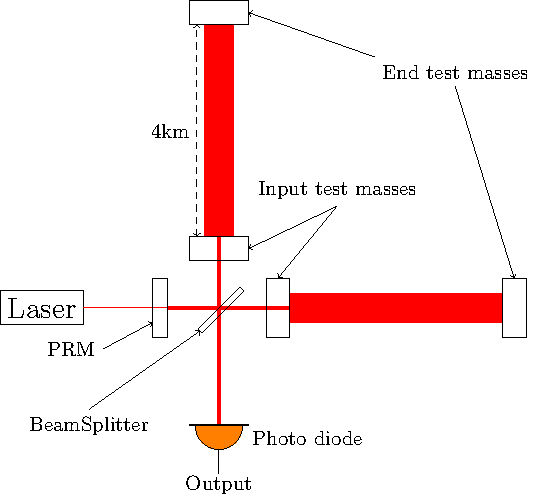
\includegraphics[width=0.5\textwidth]{chapters/foundations/sections/cbc_searches/images/michelson_interferometer.pdf}
	\caption[Diagram of a laser interferometer gravitational-wave detector]{The figure shows a simplified diagram of the interferometric \acrshort{gw} detectors. The diagram is not to scale and only highlights the beam path. Any operations for stabilization, mode cleaning, and so on are not shown. The laser beam travels from the laser through the power recycling mirror (PRM) to the beam splitter, where it is split into equal parts to the two arms. In each arm, the beam passes an input test mass, which is a mirror, travels \SI{4}{\kilo\metre}, and is reflected at the end test mass. On its way back, a large portion of the light is again reflected by the input test mass to increase the light travel time in the arms. Together the two test masses essentially create a large Fabry-Perot cavity. Once the light passes the input test mass, it recombines and interferes with the light from the other arm. A photodiode captures the beam at the output port (south) to produce the readout. The part going back to the laser is reflected at the power recycling mirror to increase the laser power in the interferometer. This figure was adapted from Figure 1 in \cite{LIGOScientific:2014pky}.}\label{fig:detector_diagram}
\end{figure}

To obtain the length deviation, one can in principle use equation \eqref{eq:geodesic_deviation_gw} as discussed above. However, that equation is in a frame of reference in which the effect of \acrshort{gw}s on test masses can be easily described and where the $x^3$ direction points from the source to the detector. The frame of reference of the detector, on the other hand, defines the $x$- and $y$-axis as the arms of the detector and the $z$-axis such that it is orthogonal to the $x$-$y$-plane pointing away from the center of the earth. To translate the motion in one frame to the motion in the other frame, one can use a transformation based on Euler-rotations. Carrying out these calculations leads to~\cite{Schutz:2011tw}
\begin{align}\label{eq:delta_l}
h = & \phantom{+}F_+\lr{\theta, \varphi}\lr{\cos\lr{2\psi}h_+ - \sin\lr{2\psi} h_\times}\nonumber\\
& + F_\times\lr{\theta, \varphi}\lr{\sin\lr{2\psi}h_+ + \cos\lr{2\psi} h_\times},
\end{align}
where $\theta$, $\varphi$, and $\psi$ are the Euler-angles known as declination, right ascension, and polarization angle, respectively, and
\begin{align}\label{eq:antenna_patterns}
F_+\lr{\theta, \varphi} & = \frac{1}{4}\lr{3+\cos\lr{2\theta}}\sin\lr{2\varphi}\nonumber\\
& = \frac{1}{2}\lr{1 + \cos^2\lr{\theta}}\sin\lr{2\varphi},\nonumber\\
F_\times\lr{\theta, \varphi} & = \cos\lr{\theta}\cos\lr{2\varphi}.
\end{align}

In total, the \acrshort{gw}s the detectors measure depend on $15$ parameters for \acrshort{bbh} signals and $17$ for \acrshort{bns} systems. An overview of these parameters is given in \autoref{fig:gw_params}. They affect the measured signal in different ways:
\begin{description}
	\item[$\bm{m_1, m_2}$] The component masses of the two objects. Usually it is defined that $m_1\geq m_2$. To leading order they are the only parameters that influence the frequency evolution of the signal and they act mainly through the mass combination known as the chirp mass. The larger the total mass of the system, the lower the frequency at which the two objects merge.
	\item[$\bm{\vec{\chi}_1, \vec{\chi}_2}$] The three-dimensional spin vectors of the individual objects. They often are only measured in a mass-weighted form known as the effective spin $\chi_e$~\cite{Schmidt:2012rh} and the effective precession spin $\chi_p$~\cite{Schmidt:2014iyl}. As long as the spins are (anti-)aligned with the orbital angular momentum, they affect the time scale at which the objects merge. The more aligned the spin, the longer the time scale. If they are not aligned with the orbital angular momentum they cause precession effects, that become visible as a beating in the signal.
	\item[$\bm{\Lambda_1, \Lambda_2}$] Tidal deformabilities of the two objects. They quantify the amount of matter distortion due to the gravitational gradient in the close proximity to a highly compact object. Subsequently they are $0$ for \acrshort{bh}s and are only considered for \acrshort{bns} and \acrshort{nsbh} mergers. The larger the tidal deformability, the stiffer the \acrshort{ns}, and the longer the duration of the inspiral. However, the influence of matter effects are expected to be very small and they have not been measured yet~\cite{LIGOScientific:2021djp}.
	\item[$\bm{r}$] The distance from the source to the detector. It is inversely proportional to the amplitude of the waveform measured in the detector.
	\item[$\bm{\theta, \varphi}$] The declination $\theta$ and the right ascension $\varphi$ in the reference frame of the detector. They affect the amplitude of the measured signal through \eqref{eq:delta_l} to the point where the detectors can be blind to specific polarizations from given locations in the sky. \autoref{fig:sky_location_influence} shows the average influence of the sky position on the strength of the detected signal.
	\item[$\bm{\Psi}$] The polarization angle. It is the angle by which the frame of the \acrshort{gw} has to be rotated around the propagation axis to line up with the frame of the detector. For a single detector it can be absorbed into a redefinition of the two polarizations of the wave and cannot be resolved. See \autoref{fig:gw_params} for a visualization of this angle.
	\item[$\bm{\iota}$] The inclination of the orbital plane of the source with respect to the line of sight of the detector. It influences the radiated power and, therefore, the amplitude of the signal. A plot of the power distribution is shown in \autoref{fig:angle_power}.
	\item[$\bm{\Phi_0}$] The coalescence phase, i.e. the orbital position of the two objects at merger. It introduces an overall phase-shift in the measured signal.
	\item[$\bm{t_0}$] The time of coalescence, which is often defined as the time at which the merger signal arrives at the center of the earth. Controls the time at which the system merges and time shifts the waveform in the detector data.
\end{description}

\begin{figure}
	\centering
	\begin{subfigure}[b]{.72\linewidth}
		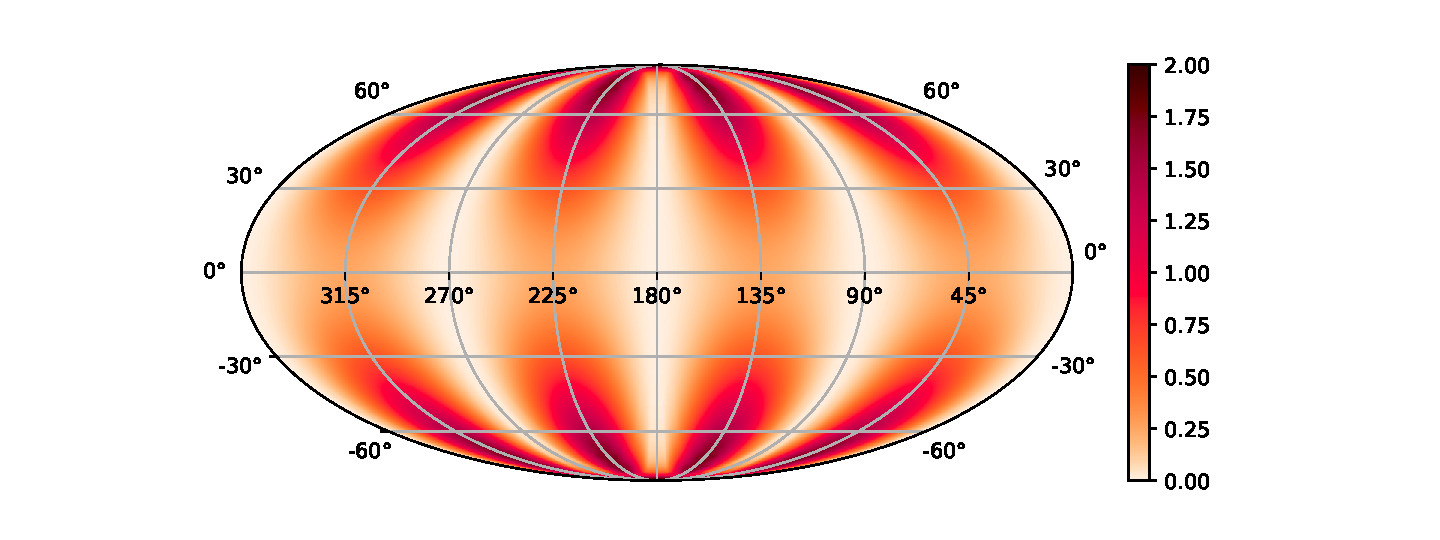
\includegraphics[width=\linewidth]{chapters/foundations/sections/cbc_searches/images/sky_location_power.pdf}
		\caption{Sky location}\label{fig:sky_location_influence}
	\end{subfigure}
	\begin{subfigure}[b]{.27\linewidth}
	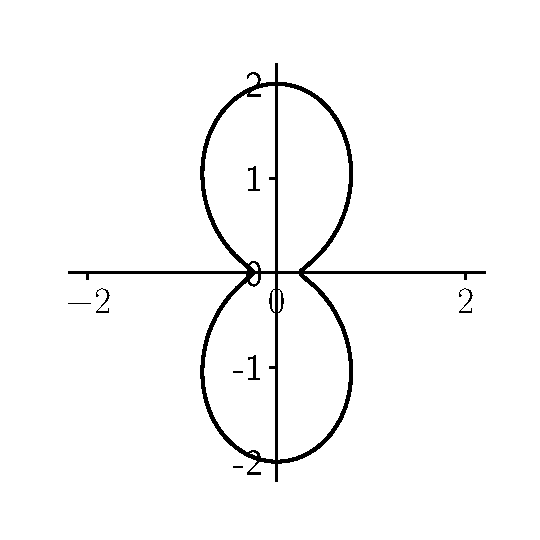
\includegraphics[width=\linewidth]{chapters/foundations/sections/cbc_searches/images/angular_power_distribution.pdf}
	\caption{Inclination}\label{fig:angle_power}
	\end{subfigure}
	\caption[Gravitational wave angular power distributions]{\textbf{(a) Sky location:} The influence of the sky-position on the \acrshort{gw} intensity observed by the detector averaged over all source orientations. It is known as the antenna power function and we observe that there are favorable and unfavorable sky-locations for the detectors. This figure was inspired by Figure 2 of \cite{Schutz:2011tw}. \textbf{(b) Inclination:} The multiplicative factor of the radiated power of a \acrshort{gw}. The angle to the x-axis is the inclination of the system, the distance to the origin gives the factor by which the radiated power from the source intrinsic parameters has to be multiplied. This shows that face-on systems ($\iota=\pi/2$ or $\iota=3\pi/2$) are seen with the highest intensity, while edge-on systems ($\iota=0$ or $\iota=\pi$) are observed with the lowest intensity. However, it also shows that there is no dead-spot and some power is radiated in all directions. This figure was adapted from Figure 3.7 of \cite{Maggiore:2008aaa}}
\end{figure}
\begin{figure}
	\centering
	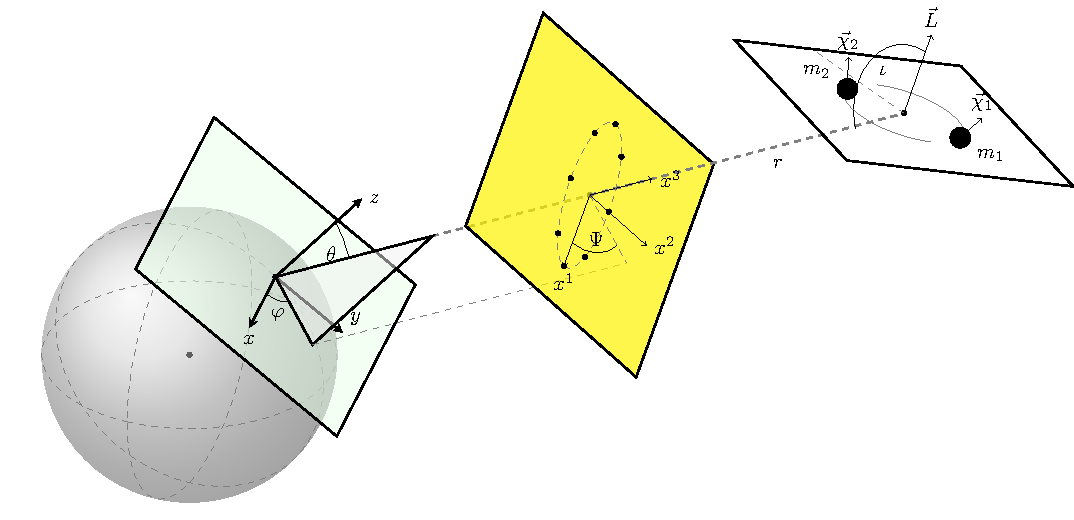
\includegraphics[width=\textwidth]{chapters/foundations/sections/cbc_searches/images/gw_params.pdf}
	\caption[Gravitational wave signal parameters]{A diagram showing the parameters the measured signal of a \acrshort{bbh} merger depends on. The three differently colored planes indicate the three different coordinate systems used in the calculation of the \acrshort{gw} effect. The white plane belongs to the source. It is aligned with the orbital plane. The yellow frame shows the preferred frame of reference for a \acrshort{gw}, where its propagation direction is aligned with the $x^3$-axis. The deformed ellipsoid on the plane indicates the movement of a ring of test masses in this frame (compare \autoref{fig:effect_gw}). The green plane shows the frame of the detector, where the $x$- and $y$-axes are aligned with the detector arms and $z$ points away from the center of the earth, which is depicted as the gray sphere. The angles show the transformations that are associated with them. The distance $r$ is highlighted by the dashed gray line connecting the detector and the source. Not shown are the time of coalescence $t_0$ and the coalescence phase $\Phi_0$. $\vec{L}$ shows the orbital angular momentum. The figure is not to scale and only meant to show the meaning of the different parameters. It was inspired by Figure 9.2 of \cite{Hawking:1989aaa}.}\label{fig:gw_params}
\end{figure}

Equation \eqref{eq:delta_l} describes the signal the detector would pick up in an ideal environment. However, as we all know the world around us is not an ideal environment, as it is noisy. To get a sense of scale at which noise sources have to be considered, one can estimate the length change induced by a \acrshort{gw} on an interferometric detector with arms at a right angle and \SI{4}{\kilo\metre} length. Using \eqref{eq:linear_waveform} for a non-spinning, face-on system ($\iota=0$) at a distance $r$ of \SI{1}{\giga\parsec} with masses similar to those of the first observed \acrshort{gw} directly overhead the detector yields a length deviation of $\approx$ \SI[parse-numbers=false]{10^{-18}}{\metre}. At these length scales almost any noise source is non-negligible. The most important noise sources are the following~\cite{Pitkin:2011yk, LIGOScientific:2014pky, VIRGO:2014yos}:
\begin{description}
 \item[Seismic noise] Seismic noise consists of small vibrations of the earth, caused by anything from passing cars to earthquakes. It is most notable at small frequencies. Along with the gravity gradient noise (see below) and control noise~\cite{Dooley:2013jqa, aLIGO:2020wna} it is the main reason why earth bound detectors are not sensitive to sub-Hertz \acrshort{gw}s (compare \autoref{fig:noise_limit}). To isolate the detector from most of the seismic noise, the mirrors are suspended in a triple pendulum setup and vertically damped by springs. A combination of active and passive isolation is deployed.
 \item[Thermal noise] Thermal noise has many sources. Any part that has a finite temperature vibrates and adds noise into the system. The most important sources are the Brownian motion of the mirror coatings and the thermal noise in the suspension used to isolate the mirrors from seismic noise. Additionally, due to the high laser-power required in the detectors, the mirrors have a temperature gradient that adds additional noise. The coating Brownian noise has a non-negligible impact in the most sensitive regions of the detector (compare \autoref{fig:noise_limit}), while the other thermal noise sources usually enter at low frequencies. To reduce thermal noise, KAGRA operates at cryogenic temperatures~\cite{KAGRA:2018plz}.
 \item[Quantum noise] Quantum noise has two origins. First, there is shot noise. This is the noise in the measured output power, due to the discrete nature of individual photons in the laser beam. Second, there is radiation pressure noise. It is caused by the laser beam exerting a pressure on the mirror. Due to the discrete nature of the photons, this pressure fluctuates. Combined, quantum noise is the limiting factor for the sensitivity in the most sensitive frequency range as well as at high frequencies. To reduce shot noise, one can increase the laser-power. However, with greater laser power, the radiation pressure noise increases and thermal effects become more prominent. Another option to reduce shot noise is the usage of squeezed light~\cite{Caves:1981hw, LIGOScientific:2013pcc, Lough:2020xft}. Squeezing can be used to shift noise from phase to amplitude, thus reducing shot noise, or vice versa to reduce radiation pressure noise by utilizing the Heisenberg uncertainty principle~\cite{Heurs:2018wsu}.
 \item[Gravity gradient noise] Gravity gradient noise is caused by seismic waves that induce density fluctuations in the earth. These density fluctuations causes the gravitational field to change over time and influence the detector. Because these shifts in density are relatively slow processes, this type of noise is large at low frequencies and is a limiting factor. Since the gravitational field cannot be shielded, the only way to reduce gravity gradient noise is to select locations for the detectors where density fluctuations are small. One can also monitor the changes in the gravitational field and subtract their influence afterward.
\end{description}

\begin{figure}
	\centering
	\begin{subfigure}[b]{.56\linewidth}
		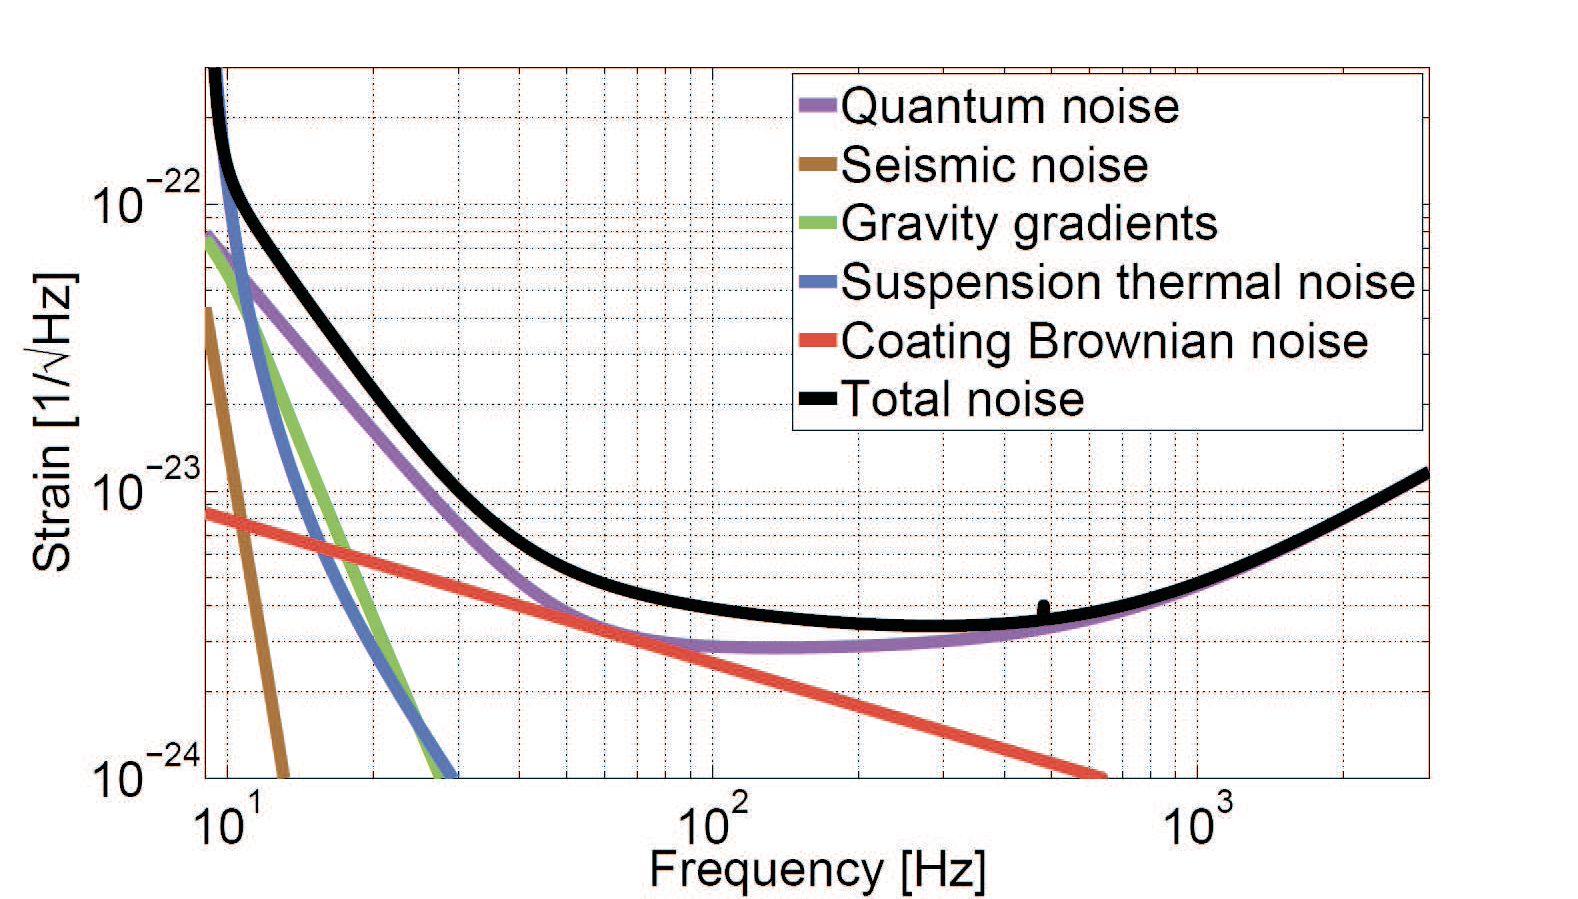
\includegraphics[width=\linewidth]{chapters/foundations/sections/cbc_searches/images/noise_limits_aligo.png}
		\caption{The noise budget of the advanced \acrshort{ligo} detectors.}\label{fig:noise_limit}
	\end{subfigure}
	\hspace{0.03\linewidth}
	\begin{subfigure}[b]{.34\linewidth}
		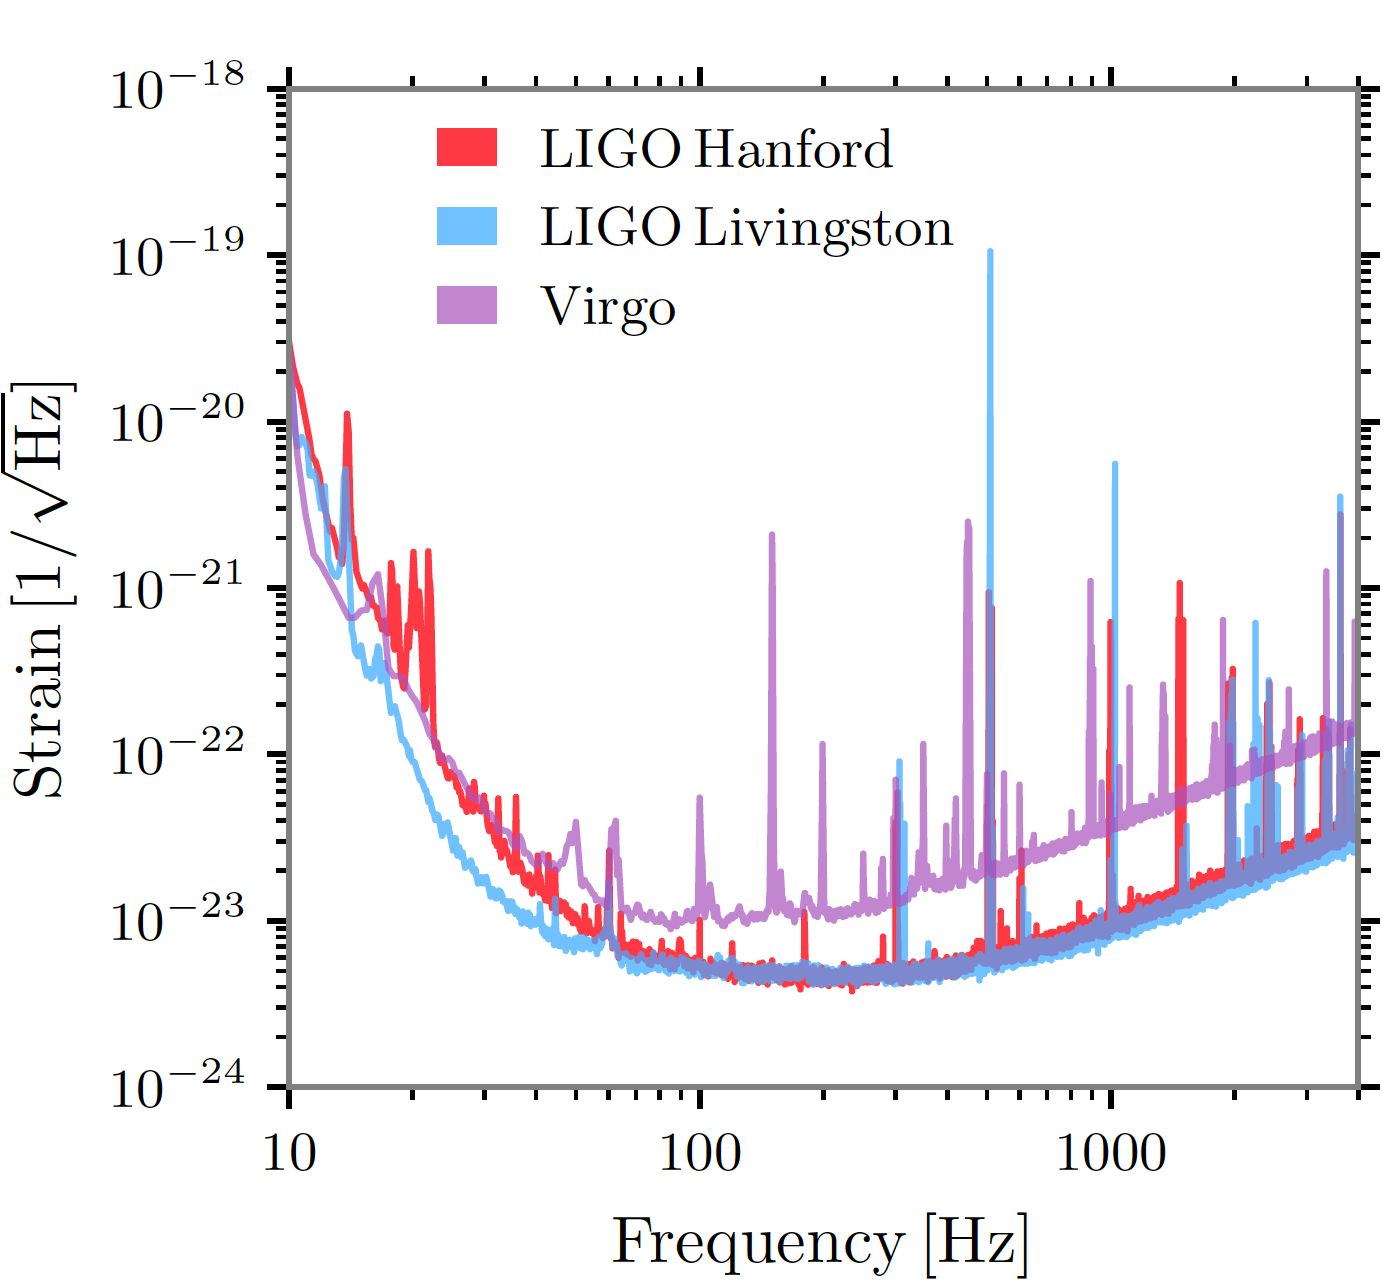
\includegraphics[width=\linewidth]{chapters/foundations/sections/cbc_searches/images/noise_o3_2.png}
		\caption{Power spectrum measured during \acrshort{o3}.}\label{fig:noise_o3}
	\end{subfigure}
	\caption[Noise amplitude spectrum]{The theoretical noise budget of the detector (a) and the measured amplitude spectrum (b) of advanced \acrshort{ligo}. The left figure shows the contribution of the different noise sources to the overall noise of the detector. It was taken from \cite{LIGOScientific:2014pky}. The right figure shows measured \acrshort{asd}s for the three main detectors during \acrshort{o3}. The curves are representative of the detector sensitivity during the observational period and the figure was taken from \cite{LIGOScientific:2021djp}.}
\end{figure}

To characterize the strength of the noise, one can calculate the \emph{power spectral density} (\acrshort{psd}). The \acrshort{psd} gives the power present in the detector due to noise as a function of the frequency. On a finite stretch of pure noise data $n\lr{t}$ with duration $T$ the one-sided \acrshort{psd} $S_n\lr{f}$ can be calculated as~\cite{Maggiore:2008aaa}%page 337
\begin{equation}
S_n\lr{f} = \frac{2}{T} \langle{\left|\tilde{n}\lr{f}\right|}^2\rangle,
\end{equation}
where $\tilde{n}\lr{f}$ is the Fourier transform of $n\lr{t}$ and the average $\langle\cdot\rangle$ is performed over different realizations of the noise. Its frequency resolution $\Delta f$ is given by $1/T$ and, by matching the units, one can infer that the \acrshort{psd} is given in units of \SI{}{1/\hertz}. In practice, the data is often chopped into many overlapping shorter pieces, a window is applied to each piece to reduce the impact of required periodicity of the Fourier transform, and the resulting \acrshort{psd}s are averaged. This algorithm is known as Welch's method~\cite{Welch:1967aaa}.

\autoref{fig:noise_o3} shows an estimate of the \emph{amplitude spectral density} (\acrshort{asd}) during the third observing run (\acrshort{o3}) for the three detectors that collected the majority of the data. The \acrshort{asd} is the square root of the \acrshort{psd}. Comparing it to the theoretical limit from \autoref{fig:noise_limit} one finds that the measured noise contains high spikes at certain frequencies. Most of these originate from known sources, such as the power grid frequency or violin modes of the mirror suspensions~\cite{LIGOScientific:2019hgc}. However, due to their narrow frequency range the effect on the detectability of \acrshort{gw}s from \acrshort{cbc} sources is marginal.

One noise characteristic that is not evident in the \acrshort{psd}s are short duration non-Gaussian noise transients known as \emph{glitches}. They can mimic the frequency evolution of real \acrshort{gw} events and a lot of effort is being invested to reject them \cite{Allen:1999yt, Allen:2004gu, Zevin:2016qwy, Robinet:2020lbf}. These glitches are by no means rare with an average glitch rate of \SIrange{0.29}{1.17}{\minute^{-1}}~\cite{LIGOScientific:2021djp}. The cause for some of these glitches is known and can be traced back for instance to light scattering or computer glitches; others have yet uncharacterized origins~\cite{Zevin:2016qwy}.

Several upgrades and extensions to the current network of ground based \acrshort{gw} detectors are planned. To extend the network in the short term future, it is planned to construct a third observatory of the advanced \acrshort{ligo} specifications in India~\cite{Iyer:2011aaa, Saleem:2021iwi}. It is scheduled to start operations around the year 2024~\cite{KAGRA:2013rdx}. The next major upgrades to the \acrshort{ligo} detectors are known as ``A+''. They are supposed to be incremental enhancements involving better light squeezing technology, bigger test masses, and improved materials, among other adjustments~\cite{LIGOScientific:2017aaa}. Beyond 2025 upgrades are still being planned but may include substantially increased laser power, a change of the laser frequency, and cryogenic operation~\cite{LIGOScientific:2017aaa}. One such proposal is named \acrshort{ligo} Voyager. Currently two new ground based detectors are being considered for constructions and are planned to become operational in the mid 2030s. These are the Einstein Telescope (\acrshort{et}) in Europe~\cite{Maggiore:2019uih} and Cosmic Explorer (\acrshort{ce}) in the United States~\cite{Reitze:2019iox}. \acrshort{et} is planned to be a triangular interferometric detector built underground. Its special shape allows to eliminate any signal from the data and be left with a pure noise channel. \acrshort{ce} plans to use an arm length of \SI{40}{\kilo\metre}.

To eliminate the low frequency limitations of earth bound observatories, two projects are developing space based detectors. The European Space Agency (\acrshort{esa}), the National Aeronautics and Space Administration (\acrshort{nasa}), and the \acrshort{lisa} Consortium are working on the Laser Interferometer Space Antenna (\acrshort{lisa})~\cite{LISA:2017pwj, ESA:2022aaa, NASA:2022aaa}. \acrshort{lisa} will be a constellation of three satellites on a heliocentric orbit following the earth. It will use time delay interferometry with an arm length of \SI{2.5}{\giga\metre} and is expected to detect \acrshort{gw}s in the sub-Hertz regime~\cite{LISA:2017pwj}. After a widely successful test of the technology known as \acrshort{lisa} Pathfinder~\cite{McNamara:2008zz, Armano:2016bkm, Armano:2018kix}, the \acrshort{lisa} mission is now scheduled to launch in 2034~\cite{ESA:2022aaa}. A second proposed space based observatory is the TianQin detector~\cite{TianQin:2015yph}. It, too, will consist of three satellites but its arm length is reduced to \SI[parse-numbers=false]{10^5}{\metre} and it will orbit the earth.

The final detection scheme I will briefly discuss are Pulsar Timing Arrays (\acrshort{pta})s~\cite{Hobbs:2008yn, Demorest:2009ex}. \acrshort{pta}s use the extreme timing accuracy of millisecond pulsars to measure large scale deviations of their arrival times over long periods. A \acrshort{gw} in the \SI{}{\nano\hertz} regime will cause these deviations to be correlated and be recoverable. They potentially allow to detect for instance the \acrshort{gw} background or other low frequency \acrshort{gw} sources. So far no signal consistent with expected \acrshort{gw}s has been recovered with high confidence~\cite{NANOGrav:2020gpb, NANOGrav:2020bcs}.


\subsection{Matched Filtering}\label{sec:matched_filtering}
As discussed in the previous subsection \ref{sec:detectors}, the output of the detectors is contaminated with large amounts of noise. To achieve optimal sensitivity, sophisticated data analysis techniques have to be used. This subsection will discuss a technique known as \emph{matched filtering}, that uses a model of the expected signal to maximize the amount of information that can be extracted from the data.

The output of the detector is a time series $d\lr{t}$ that is the sum of the noise $n\lr{t}$ and potentially an additive signal $h\lr{t}$
\begin{equation}
d\lr{t} = n\lr{t} + h\lr{t}.
\end{equation}
In the following discussion we will assume that the noise $n\lr{t}$ is stationary and Gaussian with zero mean. For real data this is only an approximation, as the noise characteristics slowly drift over time and glitches are short duration, non-Gaussian noise transients. However, the time scale of the noise drift is slow compared to the usual duration that \acrshort{cbc} signals are observable for~\cite{Kumar:2022tto}.

If one knows the signal that is hidden in the data, one can compare the data to the signal. To do so, one can convolve the expected signal, which is called the \emph{template}, with the data
\begin{align}\label{eq:concept_mf}
\lr{h\ast d}\lr{t} & = \int_{-\infty}^{\infty}\diff{\tau}\ h\lr{\tau}d\lr{t-\tau}\nonumber\\
& = \int_{-\infty}^{\infty}\diff{\tau}\ h\lr{\tau}h\lr{t-\tau} + \int_{-\infty}^{\infty}\diff{\tau}\ h\lr{\tau}n\lr{t-\tau}.
\end{align}
In this calculation, the first integral in the second line is positive definite when the template and the signal are aligned correctly, i.e. when $t=0$. Therefore, equation \eqref{eq:concept_mf} will yield larger values in the presence of the signal $h$ than in its absence. This is the core concept behind matched filtering.

\autoref{fig:detector_data_raw} shows a short time slice of data collected during \acrshort{ligo}s first observing run (\acrshort{o1}) and the \acrshort{asd} calculated from the detector data $d$ on a \SI{32}{\second} interval around the shown slice. The \acrshort{asd} shows that the detector noise is dominated by low frequencies, which becomes evident by the slow oscillations with large amplitudes in the left panel of \autoref{fig:detector_data_raw}. However, this also tells us that signals at low frequencies are much more likely to be overshadowed by noise. Therefore, one can downweigh frequencies where the detector is particularly noisy.

\begin{figure}
	\centering
	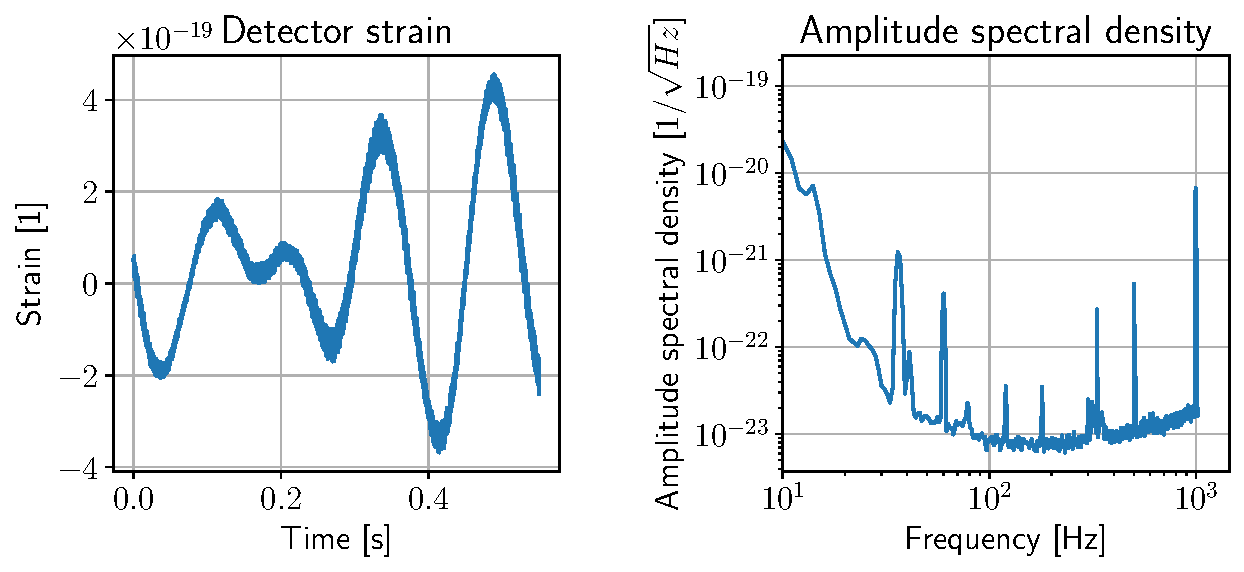
\includegraphics[width=0.98\textwidth]{chapters/foundations/sections/cbc_searches/images/data_raw.pdf}
	\caption[Raw detector data]{A small slice of raw detector data from the Gravitational Wave Open Science Center (\acrshort{gwosc}) (left) and the corresponding \acrshort{asd} (right). The \acrshort{asd} was calculated from \SI{32}{\second} around the shown data slice using Welch's method with a window duration of \SI{1}{\second} and a step size of \SI{0.5}{\second} between the windows~\cite{LIGOScientific:2019lzm}.}\label{fig:detector_data_raw}
\end{figure}

In practice this process is called \emph{whitening}, as it attempts to scale the power at each frequency to be $1$. Noise which has a flat \acrshort{psd} is known as white noise. This can be achieved by dividing the Fourier transformed data $\tilde{d}\lr{f}$ by the \acrshort{asd}
\begin{equation}
\hat{d}\lr{t} = \int \diff{f}\ \frac{\tilde{d}\lr{f}}{\sqrt{S_n\lr{f}}} e^{i2\pi ft}.
\end{equation}
This operation in the time domain is a convolution of the data $d$ with a filter $F^{-1}\lr{1/\sqrt{S_n\lr{f}}}$, where the function $F^{-1}$ represents the inverse Fourier transform. Due to high peaks in the \acrshort{asd} at some frequencies, the filter has non-negligible power even at times far away from zero. Since the Fourier transform assumes the data to be periodic, the long duration of the filter correlates independent data points and corrupts the data. To avoid this corruption the filter is truncated in the time domain to a finite duration, by applying a window that tapers to zero. The corruption is, thereby, limited to half the truncated duration of the filter in the beginning and end of the whitened data. The corrupted parts of the data are subsequently cropped. By truncating the whitening filter in the time domain, the sharp frequency lines of the \acrshort{asd} are broadened which is usually not a problem for \acrshort{cbc} signal detection.

\autoref{fig:detector_data_white} shows the same data as \autoref{fig:detector_data_raw} but with whitening applied to it. The \acrshort{asd} is now almost flat and has a value of $\approx 1$ at each frequency. Looking closely, one can start to make out a waveform around \SI{0.4}{\second} from the start of the data. Cropping to remove edge effects was applied outside of the shown window.

\begin{figure}
	\centering
	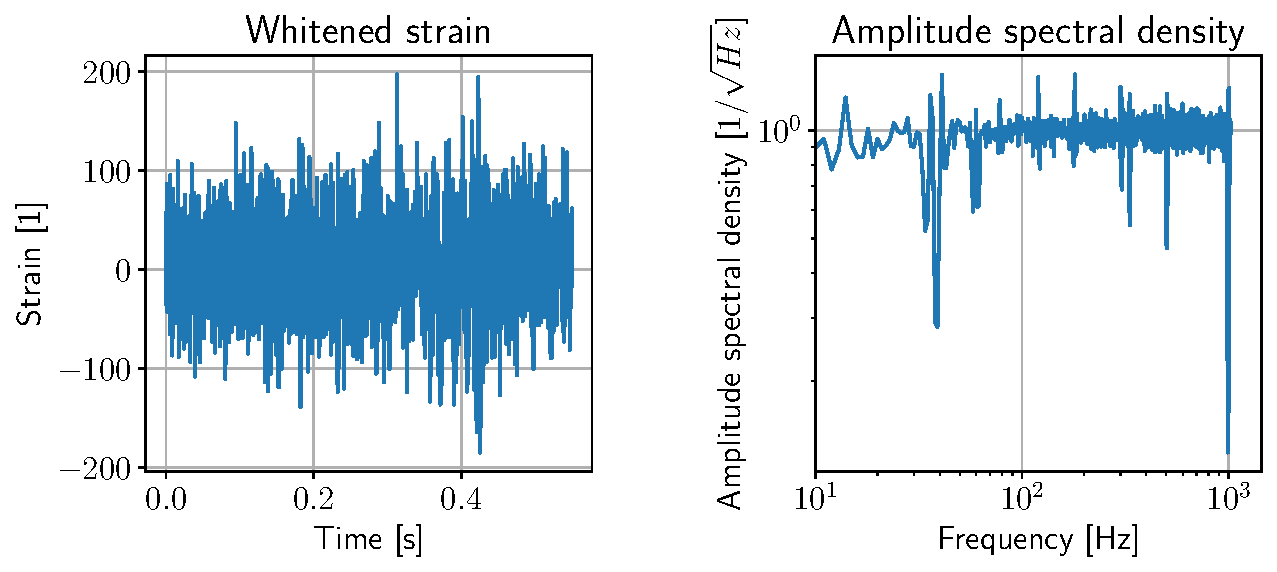
\includegraphics[width=0.98\textwidth]{chapters/foundations/sections/cbc_searches/images/data_white.pdf}
	\caption[Whitened detector data]{The data shown in \autoref{fig:detector_data_raw} whitened by the associated \acrshort{psd} (left) and the \acrshort{asd} calculated on the whitened data (right). The entire \SI{32}{\second} of data were whitened. Therefore, edge effects are clipped from the shown data slice.}\label{fig:detector_data_white}
\end{figure}

Using the whitened data and an accordingly whitened template in \eqref{eq:concept_mf} maximizes the difference between the value obtained when filtering pure noise and noise with the template added into it~\cite{Maggiore:2008aaa}. It is mathematically proven to be the optimal filter for stationary Gaussian noise~\cite{Allen:2005fk}. Since the data and template are transformed to the Fourier domain to whiten them and since the convolution operation can be expressed by a multiplication in the Fourier domain, the matched filter is given by~\cite{Maggiore:2008aaa, Usman:2015kfa}% page 345
\begin{equation}
\rho\lr{t} = \frac{\langle h\vert d\rangle}{\sqrt{\langle h\vert h\rangle}},
\end{equation}
where
\begin{equation}\label{eq:mf_inner_product}
\langle a\vert b\rangle\lr{t} = 4\text{Re}\left[\int_0^\infty\diff{f}\ \frac{\tilde{a}^\ast\lr{f}\tilde{b}\lr{f}}{S_n\lr{f}} e^{i2\pi ft}\right].
\end{equation}
The factor $\sqrt{\langle h\vert h\rangle}$ is used for normalization and the factor $4$ comes from using the one-sided \acrshort{psd} as well as taking the integral of the symmetric argument from $0$ instead of $-\infty$. The function $\text{Re}\left[\cdot\right]$ extracts the real part of a complex number. The function $\rho\lr{t}$ is the \emph{signal-to-noise ratio} (\acrshort{snr}). When the \acrshort{snr} exceeds a threshold, which is determined by search configurations, the search has potentially identified the signal.

So far it was assumed that the signal in the data is known. In reality this assumption does not hold, as we do not even know if a signal is present and if one is present, what kind of system emitted it. However, matched filtering is highly sensitive to the phase of the signal. This means that when the phases of the template and the actual signal deviate by even a moderate amount, the \acrshort{snr} drops significantly. For this reason, one usually constructs a \emph{template bank}, that covers a specified region of possible parameters. It is constructed by requiring that the \emph{match} between two neighboring templates does not fall below a given limit. The match is the inner product \eqref{eq:mf_inner_product} of the two signals, maximized over the phase and coalescence time, and normalized by the norm induced by the inner product \eqref{eq:mf_inner_product} of both templates. Usually matches $\geq 0.95$ are required~\cite{LIGOScientific:2021djp, Nitz:2021uxj}.

The data has to be filtered against every template in the bank. Therefore, the computational cost scales linearly with the number of templates. However, the number of templates scales exponentially with the number of degrees of freedom in the system. For this reason, it is desirable to reduce the dimensions of the parameter space as much as possible. To do so, searches make a series of assumptions and optimizations. First, search template banks are usually constructed using only the dominant $22$-mode. This means that equation \eqref{eq:complex_waveform} essentially reduces to
\begin{equation}
H = h_+ + i h_\times = A\lr{\tau, r, \iota, \Phi_0, \kappa} e^{-i\Phi\lr{\tau, \kappa}}.
\end{equation}
Second, by using
\begin{equation}
h_+ = \frac{H + H^\ast}{2},\ \quad
h_\times = \frac{H - H^\ast}{2i}
\end{equation}
in \eqref{eq:delta_l} one finds that the measured strain in the detector is of the form~\cite{Allen:2005fk}
\begin{equation}\label{eq:qualitativ_detector_output}
h = \text{Re}\left[\frac{A\lr{\tau, \kappa}}{D_\text{eff}\lr{r, \theta, \phi, \psi, \iota}}\exp\lr{-i\lr{2\Delta\Phi\lr{\theta, \phi, \psi, \iota, \Phi_0} + 2\Phi\lr{\tau, \kappa}}}\right].
\end{equation}
$D_\text{eff}$ is known as the effective distance and quotes the distance at which the same source could be seen with the same amplitude, assuming an optimal orientation and a location directly overhead the detector. An explicit expression for $D_\text{eff}$ can be found in \cite{Allen:2005fk}. $\kappa$ represents all source internal parameters, i.e. the masses, spins, and tidal deformabilities. From \eqref{eq:qualitativ_detector_output} we find that the source location and orientation with respect to the detector introduce a time independent phase shift and scale the amplitude. The amplitude scaling can be combined with the distance $r$ to form a single parameter; the effective distance. Observing a source in one location has the same amplitude evolution as observing the same source at the optimal location and orientation, just at a farther distance. The phase shift on the other hand can be combined with the coalescence phase, to form a second effective parameter. So instead of being concerned with the $4$ parameters $\theta$, $\phi$, $\psi$, and $\iota$, all of them can be absorbed into the distance $r$ and coalescence phase $\Phi_0$. The distance, on the other hand, sets a normalized scale for the \acrshort{snr} and, therefore, does not need to be included in the template bank~\cite{Allen:2005fk}. The coalescence phase can also be eliminated from the template bank, by maximizing the \acrshort{snr} over it. If the projection onto the real axis in \eqref{eq:mf_inner_product} is removed, the \acrshort{snr} time series becomes complex. An overall phase shift in the template rotates the \acrshort{snr}-vector in the complex plane, but does not change its length. So by taking the absolute value of the \acrshort{snr} time series, one maximizes its value over the coalescence phase, irrespective of the phase value. This is equivalent to using the total \acrshort{snr} by combining the \acrshort{snr} of filtering with the template $h$ and its phase shifted counterpart $ih$~\cite{Allen:2005fk, Ohme:2012cba, Usman:2015kfa}
\begin{equation}
\rho_{\Phi_{0,\text{max}}}\lr{t} = \sqrt{\frac{{\langle h\vert d\rangle}^2+{\langle ih\vert d\rangle}^2}{\langle h\vert h\rangle}}.
\end{equation}

Third, template banks usually assume non-precessing systems~\cite{LIGOScientific:2021djp, Nitz:2021zwj}. This reduces the dimensionality of the parameter space even further, as the original $6$ spin parameters are reduced to a total of $2$ values that need to be covered. Finally, the inverse Fourier transform in \eqref{eq:mf_inner_product} is equivalent to doing a convolution of the data with a template. So it efficiently changes the coalescence time $t_0$ of the template and produces the \acrshort{snr} value for all possible values. All these optimizations lead to a four dimensional space that needs to be covered by the template bank; $m_1$, $m_2$, $\chi_1^3$, $\chi_2^3$.

Current standard searches are limited to systems with aligned spin and a mass range from $\approx$ \SI{1}{M_\odot} to $\approx$ \SI{500}{M_\odot}, depending on the implementation~\cite{LIGOScientific:2021djp, Nitz:2021uxj}. Lower masses require denser template banks, as the systems are within the sensitive band of the detectors for a larger number of cycles. This allows small phase errors to accumulate to the point where match requirements are exceeded~\cite{Harry:2009ea}. The high-mass region is rather limited by the short duration, which makes it difficult to distinguish astrophysical signals from glitches~\cite{Nitz:2017lco}.

Although using matched filtering alone is sufficient to detect \acrshort{gw}s, it is often stated that the first detected \acrshort{gw} is visible in the data with the naked eye. While one can barely make something out in \autoref{fig:detector_data_white}, we can make use of the fact that we know the frequencies of the signal. \autoref{fig:detector_data_bandpassed} shows the data after whitening and applying an additional bandpass filter for the range \SIrange{20}{256}{\hertz}. The signal is now clearly visible in the time domain data.

\begin{figure}
	\centering
	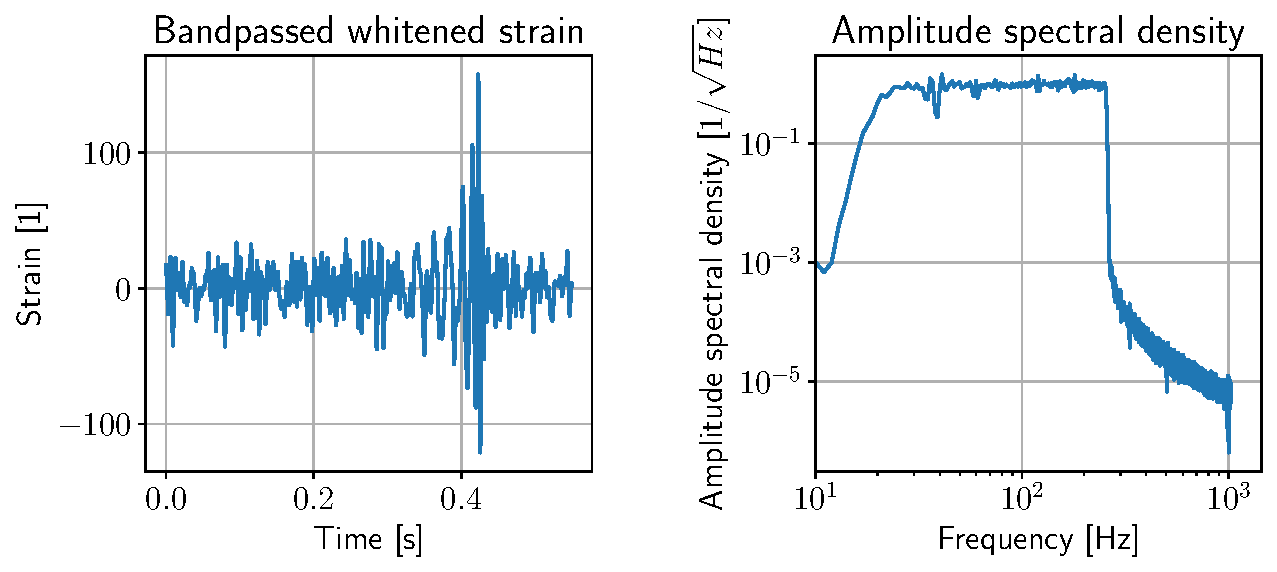
\includegraphics[width=0.98\textwidth]{chapters/foundations/sections/cbc_searches/images/data_bandpassed.pdf}
	\caption[Bandpassed and whitened detector data]{The whitened data from \autoref{fig:detector_data_white} with a highpass filter of \SI{20}{\hertz} and a lowpass filter of \SI{256}{\hertz} applied (left). The corresponding \acrshort{asd} is shown on the right. The signal is now clearly visible. The data for all of these figures is the Hanford data around GW150914~\cite{LIGOScientific:2016aoc}.}\label{fig:detector_data_bandpassed}
\end{figure}

Since matched filtering is mathematically proven to be the optimal descriminator between pure noise and noise plus signal~\cite{Allen:2005fk}, it is used as a target for the deep learning detection algorithms discussed in this thesis.

This section discussed detection algorithms based on matched filtering. Due to heavy optimization, these algorithms are not designed to make statements about many of the interesting parameters of the source. The task of extracting all parameters that influence the waveform from the data is called \emph{parameter estimation}. These algorithms explore the likelihood surface and allow to give estimates of the parameters of the source and quantify them with error bars. Since the likelihood usually has to be estimated for millions of points, these algorithms are computationally very expensive and can take days or even weeks to converge. For a deeper explanation see for instance \cite{LIGOScientific:2016vlm, Biwer:2018osg, LIGOScientific:2019hgc}.


\subsection{Search Algorithm and Significance of Detections}
The matched filter of the previous subsection produces a \acrshort{snr} time series for every template. These are numerical values where larger values usually imply a greater certainty that a \acrshort{gw} is present in the data. Values of this kind are known as \emph{ranking statistic}. The question a detection pipeline has to answer is: What value of the ranking statistic is required for us to be confident that we have detected a \acrshort{gw}? This subsection will go into how this question is answered. I will follow the order of steps used by the PyCBC offline analysis~\cite{Usman:2015kfa} but note that other modeled pipelines conceptually work the same way and only differ in details~\cite{Messick:2016aqy, Adams:2015ulm}.

The first step a search pipeline has to perform is to select the data that should be analyzed. The noise characteristics of the detectors change over time~\cite{LIGOScientific:2019hgc}. During some periods, the data quality drops to a level where analysis would lead to excessive rates of false positive detections. For this reason, these parts of the data are identified by high-level quality checks~\cite{LIGO:2021ppb} and excised from the analysis data. Easily identifiable loud glitches are also cropped from the data~\cite{LIGO:2021ppb}. The overall shape of the stationary component of the noise is estimated by calculating the average \acrshort{psd} for each detector and an appropriate template bank is constructed~\cite{Usman:2015kfa}.

Afterward, the data from all detectors are filtered against the template bank to produce \acrshort{snr} time series. From there, candidate events are identified by applying a simple threshold to the \acrshort{snr} time series. The resulting points are subsequently clustered for each template, as especially loud signals usually exceed the threshold for multiple samples. The cluster window duration is a free parameter, which has to be small compared to the expected time between signals and subsequent glitches.

If the noise in the detector were stationary and purely Gaussian, one could take the \acrshort{snr} values of the candidate events as a ranking statistic. However, as discussed in subsection \ref{sec:detectors} the noise is frequently contaminated with glitches. Those that have not been removed from the data can lead to large \acrshort{snr} values, even when the underlying process that produced the transient has little to no resemblance to the signal one is searching for. Therefore, the \acrshort{snr} is usually augmented with additional statistics to form the ranking statistic. The goal of these additional statistics is to reduce the value of the ranking statistic for glitches, i.e. down weighting their influence.

The most common adaptation is to to check the data for consistency with the template. PyCBC and MBTA use a $\chi^2$-test that checks if the evolution of the potential signal matches the expected signal evolution in different time- and frequency-bands~\cite{Allen:2004gu, Usman:2015kfa, Adams:2015ulm}. GstLAL uses a $\xi^2$-test that checks the evolution of the \acrshort{snr} time series against the expected evolution~\cite{Messick:2016aqy}. More recently, efforts were made to include the short term fluctuations of the \acrshort{psd} into the ranking statistic~\cite{Venumadhav:2019tad, Nitz:2020oeq}. This reduces the impact of a less stationary detector on the trigger rate.

Once the triggers and their corresponding ranking statistics have been determined for each detector individually, they are checked for coincidences between multiple observatories. A signal from an astrophysical source has to be present in all detectors and arrival times may not differ by more than the time of flight difference between the detectors. Additionally, coincident triggers must be generated from the same template and the amplitude and phase evolution must be consistent with the time delay between the detectors~\cite{Nitz:2017svb}. These criteria already eliminate many false detections caused by glitches or other noise processes. For surviving triggers, the single detector ranking statistics are combined into a coincident ranking statistic. In recent works the coincident ranking statistic was further altered by incorporating information on the expected noise and signal trigger rates for different source parameters~\cite{Nitz:2017svb}.

As a final step, the search algorithm has to relate the numerical value of the coincident ranking statistic to a measure of how confident we are to have detected a \acrshort{gw}. In other words, the analysis must check how often a false detection is made at a given ranking statistic value. The number of false positive detections per unit time is known as the \emph{false-alarm rate} (\acrshort{far}). It is estimated by analyzing constructed background data. The background data is constructed by time shifting the single detector triggers of one detector by a duration longer than the time of flight difference between the detectors. This way, any coincident trigger cannot be of astrophysical origin. By applying multiple different time shifts, the theoretical amount of data which can only contain false positives can be extended to millions of years~\cite{Usman:2015kfa}. To determine the \acrshort{far} at a ranking statistic, the number of false positives with a coincident ranking statistic larger than the threshold are counted and divided by the theoretical duration of the analyzed data:
\begin{equation}
\mathcal{F}_\rho = \frac{N_\rho}{T}.
\end{equation}
Here $\mathcal{F}_\rho$ is the \acrshort{far} for the coincident ranking statistic $\rho$, $N_\rho$ is the number of false positives in the background with a ranking statistic $\geq\rho$, and $T$ is the duration of the analyzed background.

This thesis is mainly concerned with the comparison of machine learning based search algorithms against matched-filter based searches. For this comparison, one can analyze a simulated population of sources with both algorithms and study how many signals are recovered by either search. However, for a fair comparison we want to assess the sensitivities at the same useful astrophysical \acrshort{far}. Furthermore, to allow for an objective comparison between different works, the sensitivity must be normalized to the population. In the extreme case, the number of detected sources can always be driven to zero by choosing a population of signals injected into the noise where all sources are excessively far away. For these reasons, all works discussed in this thesis estimate the sensitive distance of the search for sensible populations. I will briefly introduce it here.

Let $\Phi\lr{\vec{x}, \lambda}$ be the probability distribution that describes the injected population, where $\vec{x}$ is the location in space and $\lambda$ are the remaining source parameters. Let, further, $\epsilon\lr{\vec{x}, \lambda; \mathcal{F}}$ be the fraction of injections being recovered by the search with parameters $\vec{x}$ and $\lambda$ with \acrshort{far} $\leq\mathcal{F}$. Then the expectation value of the volume from which sources are detected is given by~\cite{Usman:2015kfa}
\begin{equation}
\langle V\lr{\mathcal{F}}\rangle = \int \Diff{3}{x}\diff{\lambda}\ \frac{\Diff{3}{V\lr{\vec{x}}}}{{\diff x}^3}\Phi\lr{\vec{x}, \lambda}\epsilon\lr{\vec{x}, \lambda; \mathcal{F}},
\end{equation}
where $\frac{\Diff{3}{V\lr{\vec{x}}}}{{\diff x}^3}$ is the differential volume element. This volume is usually measured empirically, by applying the search to data with many known injections drawn from the distribution $\Phi$. The integral can then be estimated by Monte-Carlo integration. If the prior is uniform in volume, the sensitive volume is proportional to counting the recovered injections. This counting statistic then needs to be normalized to the prior volume and the number of injections. If the prior volume is a sphere with radius $r_\text{max}$ where injections are distributed uniformly in volume, the Monte-Carlo approximation of the sensitive volume is given by~\cite{Usman:2015kfa}
\begin{equation}
\langle V\lr{\mathcal{F}}\rangle\approx V\lr{r_\text{max}}\frac{N_{I, \mathcal{F}}}{N_I},
\end{equation}
where $N_{I, \mathcal{F}}$ is the number of injections recovered from the data with \acrshort{far} $\leq \mathcal{F}$, $N_I$ is the total number of injections in the data, and $V\lr{r_\text{max}}$ is the volume of a sphere with radius $r_\text{max}$. When a different distribution is used to sample the injections, the formula has to be reweighted or the integral has to be computed. The sensitive distance is defined as the radius of a sphere with volume $\langle V\lr{\mathcal{F}}\rangle$. As such, it is the average distance from which the search can detect sources and not an upper limit.
